\section{Algoritmo e estruturas de dados}

\subsection{Fonte de dados}
Durante a implementação do projeto, um objetivo foi manter a rotina principal (treinamento, cálculo de probabilidade dos tópicos e semelhança entre documentos) independente dos dados de treinamento e também dos dados de teste. O motivo disto é tirar o acoplamento da estrutura dos dados, do conteúdo e da forma como é feita a coleta.

Para isto foi proposta uma estrutura de dados onde foi definido o conceito de fonte de dados, que faz com que qualquer origem de dados escolhida pudesse ser trabalhada sem mudança no código fonte do algoritmo de recomendação.

Uma fonte de dados é uma abstração que tem como funcionalidade carregar os documentos de algum lugar e disponibilizar para o algoritmo de treinamento. Para ficar genérico foi criada a classe \textit{FonteDados} contendo o contrato de uma fonte, ou seja, quais métodos uma classe concreta precisa ter para fornecer os dados que o algoritmo precisa para o treinamento e também para montar o resultado com a semelhança entre os textos.

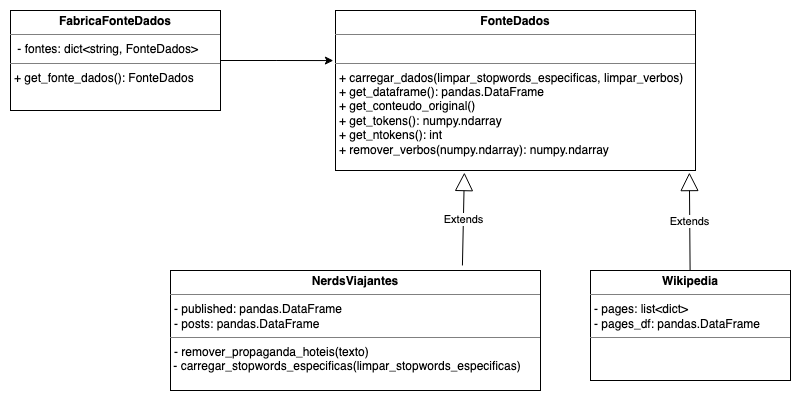
\includegraphics[scale=0.5]{fonte_dados.png}

Cada fonte de dados específica deve internamente carregar os dados e manter uma estrutura interna de forma a fornecer os documentos quebrados por tokens (palavras), assim como fornecer também um DataFrame contendo os seguintes dados:

\begin{itemize}
    \item id\_documento: id do documento na fonte de dados
    \item nome: nome do documento na fonte de dados
    \item titulo: titulo descritivo do documento na fonte de dados
    \item documento: conteudo original do documento
    \item n\_characters: tamanho do documento em caracteres
    \item tokens: tokens do documento apos limpeza
    \item n\_tokens: tamanho do documento em tokens
\end{itemize}

Desta forma as fontes de dados fornecem os dados de forma semelhante e podemos trabalhar com qualquer mídia e o algoritmo de recomendação não precisa ser alterado.
Para trabalhar com uma nova fonte de dados bastaria implementar uma subclasse de \textit{FonteDados} e implementar a parte específica que carrega os dados, faz limpeza e retorna os tokens e o DataFrame com os dados dos documentos.

\subsection{Treinamento LDA}

O módulo de treinamento LDA é responsável por ajustar um modelo para determinação de tópicos para os documentos de um conjunto de textos, assim como as 
palavras que mais contribuem para a formação de cada tópico. Recebe como parâmetros os documentos, o número de tópicos a serem escolhidos, 
além dos parâmetros do LDA passes, alpha e eta já explicados na seção de treinamento.

O treinamento consiste nos seguintes passos:

\begin{enumerate}
    \item Criar um dicionário com o conjunto total de palavras de todos os documentos. Este dicionário contém um mapeamento de um id interno para cada palavra
    \item Com base no dicionário, cria um \textit{corpus}, que é um mapeamento de frequência de ocorrência de cada palavra no conjunto inteiro de textos
    \item Faz o treinamento do modelo usando a classe \textit{LdaModel} do pacote \textit{gensim}
    \item Retorna como resultado do treinamento uma tupla com três elementos:
    \begin{itemize}
        \item Dicionário de palavras
        \item \textit{corpus}
        \item Resultado do modelo treinado
    \end{itemize}
\end{enumerate}

Segue o fragmento de código que faz este trabalho de treinamento:
\vspace{3mm} %3mm vertical space

\begin{lstlisting}[language=Python, style=mystyle, frame=lines, caption=Código fonte: Treinamento de modelo usando LDA]
    def ajustar_modelo(self, documentos, alpha=1e-2, eta=0.5e-2):
        # Cria dicionario
        id2word = dicionario.criar(documentos)

        # Cria corpus com base nos documentos e no mapeamento de id para palavra
        # Para cada documento faz a contagem de vezes que um determinado topico
        # aparece no documento
        corpus = [id2word.doc2bow(documento) for documento in documentos]

        print(f'Ajustando modelo com {self.num_topics} topicos e {self.passes} passes')

        # Treina modelo LDA        
        lda = LdaModel(corpus=corpus, id2word=id2word, 
                num_topics=self.num_topics, passes=self.passes, 
                alpha=alpha, eta=eta,
                random_state=0)

        return ResultadoTreinamentoLda(id2word, corpus, lda)
\end{lstlisting}

Para referência, um link do \href{https://github.com/heldergr/tcc-pucmg-2/blob/main/src/python/notebooks/treinamento/treinamento_lda.py}{código fonte do módulo de treinamento}.

\subsection{Cálculo de semelhança}

\subsection{Executor}

Foi criado um módulo executor para que pudessem ser variados os parâmetros de ajustes do modelo e gerar resultados para cada conjunto gerado por esta variação, permitindo uma comparação posterior dos resultados obtidos.
Este módulo recebe como parâmetro uma lista de cenários de testes. Cada cenário contém as informações:
\begin{itemize}
    \item fonte de dados de origem
    \item fonte de dados de destino
    \item topics
    \item alpha
    \item eta
    \item passes
\end{itemize}

Para cada combinação destes valores é feito o ajuste de modelo para os documentos de origem e o cálculo do documento de destino mais semelhante de 
cada documento de origem com base nas probabilidades que o documento contenha cada tópico.

\begin{comment}
    \lstinputlisting[language=Python, style=mystyle, frame=lines, caption=Código fonte: Cálculo de coerência de tópicos]{"/home/helder/estudos/tcc-pucmg-2/src/python/notebooks/main/executor.py"}
\end{comment}

Para referência, um link do \href{https://github.com/heldergr/tcc-pucmg-2/blob/main/src/python/notebooks/main/executor.py}{código fonte do executor de treinamento}.

O resultado gerado é um DataFrame com as seguintes colunas:

\begin{itemize}
    \item id\_cenario: identificador do cenário de testes
    \item fonte\_origem: descrição da fonte de origem
    \item id\_documento\_origem: identificador do documento na fonte de origem
    \item titulo\_documento\_origem: título do documento na fonte de origem
    \item fonte\_destino: descrição da fonte de destino
    \item id\_documento\_destino: identificador do documento na fonte de destino que tem a menor distância para o da fonte de origem referenciado na coluna id\_documento\_origem
    \item titulo\_documento\_destino: título do documento na fonte de destino
    \item distancia\_destino: distância calculada entre o documento na fonte de origem e o docmento na fonte de destino
    \item num\_topics: número de tópicos utilizado no modelo ajustado
    \item passes: parâmetro passes do algoritmo LDA
    \item eta: parâmetro eta do algoritmo LDA
    \item alpha: parâmetro alpha do algoritmo LDA
\end{itemize}
